\documentclass[12pt]{fphw}
%\usepackage{mathpazo}
%\usepackage[utf8]{inputenc}
%\usepackage[T1]{fontenc}
\usepackage{sectsty}
\usepackage{graphicx}
\usepackage{booktabs}
\usepackage{listings}
\usepackage{enumerate}
\usepackage{xcolor}

\sectionfont{\bfseries\large\raggedright}

\definecolor{codegreen}{rgb}{0,0.6,0}
\definecolor{codegray}{rgb}{0.5,0.5,0.5}
\definecolor{codepurple}{rgb}{0.58,0,0.82}
\definecolor{backcolour}{rgb}{0.95,0.95,0.92}

\title{Experiment 1}
\author{Aditya Kumar (24MAI14003)\\}
\date{01 Aug, 2024}
\institute{Chandigarh University\\Master of Engineeing---Artificial Intelligence}
\class{Artificial Intelligence Lab (24CSH-621)\\}
\professor{Manjit Singh}

\begin{document}

\maketitle

\section*{}
\begin{problem}
  \textbf{Aim: }Implement Uninformed Search Strategies: BFS, DFS and ID (Iterative Deepening) Ideas of Game Searching (Chess, Checkers, Tic Tac Toe, Puzzle Game, etc). 
\end{problem}
\begin{flushleft}
\section{Task to be done}
\end{flushleft}
To implement uninformed search strategies:
\begin{enumerate}
  \item BFS (Breadth-First Search)
  \item DFS (Depth-First Search)
  \item ID (Iterative Deepening)
\end{enumerate}

\section{Theory}
\textbf{BFS (Breadth-First Search)} – BFS is a fundamental algorithm used to explore or search through graphs or tree structures.

\textbf{DFS (Depth-First Search)} – DFS is another fundamental algorithm used to explore or search through graphs or tree structures. Unlike Breadth-First Search (BFS), which explores level by level, DFS explores as far down a branch as possible before backtracking.

\textbf{ID (Iterative Deepening)} – ID combines the depth-first search (DFS) strategy with a breadth-first approach, effectively balancing the benefits of both. It's particularly useful in scenarios where the depth of the solution is not known in advance, such as in certain search problems and puzzles.

\section{Algorithm}
\begin{enumerate}
  \item \textbf{Algorithm for Breadth-First Search (BFS):}
    \begin{enumerate}
      \item Initialization:
        \begin{itemize}
          \item Create an empty queue
          \item Create an empty set or list to keep track of visited nodes
          \item Enqueue the starting node and mark it as visited
        \end{itemize}
      \item Process:
        \begin{itemize}
          \item While the queue is not empty 
            \begin{enumerate}
              \item Dequeue a node from the front of the queue
              \item Process the node 
              \item For each neighnor of the node
                \begin{itemize}
                  \item If the neighbor has not been visited
                    \begin{enumerate}
                      \item Mark the neighbor as visited
                      \item Enqueue the neighbor
                    \end{enumerate}
                \end{itemize}
            \end{enumerate}
        \end{itemize}
    \end{enumerate}
  \item \textbf{Algorithm for Depth-First Search}
    \begin{enumerate}
      \item Initialization
        \begin{itemize}
          \item Create a set or list to keep track of visited nodes
          \item Call the recursive DFS function starting from the root node 
        \end{itemize}
      \item Process (Recursive DFS)
        \begin{itemize}
          \item If the node has not been visited
            \begin{enumerate}
              \item Mark the node as visited
              \item Process the node (e.g., print it, check for a condition, etc.)
              \item For each neighbor of the node 
                \begin{itemize}
                  \item If the neighbor has not been visited
                    \begin{itemize}
                      \item Recursively call DFS on the neighbor
                    \end{itemize}
                \end{itemize}
            \end{enumerate}
        \end{itemize}
    \end{enumerate}
  \item \textbf{Algorithm for Iterative Deepening (ID)}
    \begin{enumerate}
      \item Initialization
        \begin{itemize}
          \item For each depth from 0 to a specified maximum depth 
          \item Call the depth-limited DFS function with the current depth
        \end{itemize}
      \item Depth-Limited DFS 
        \begin{itemize}
          \item If the current depth is 0 and the node has not been visited
            \begin{enumerate}
              \item Mark the node as visited
              \item Process the node 
            \end{enumerate}
          \item If the current depth is greater than 0 
            \begin{enumerate}
              \item Mark the node as visited
              \item For each neighbor of the node 
                \begin{itemize}
                  \item If the neighbor has not been visited
                    \begin{itemize}
                      \item Recursively call depth-limited DFS on the neighbor with depth reduced by 1
                    \end{itemize}
                \end{itemize}
            \end{enumerate}
        \end{itemize}
    \end{enumerate}
\end{enumerate}

\section{Pseudocode}
\begin{enumerate}
  \item \textbf{Breadth-First Search (BFS)}
    \begin{lstlisting}[language=Python, tabsize=2]
BFS(graph, start_node):
    Initialize an empty queue
    Initialize a set for visited nodes
    Enqueue the start_node and mark it as visited
    
    while queue is not empty:
        node = dequeue from queue
        process the node
        
        for each neighbor of node:
            if neighbor is not visited:
                mark neighbor as visited
                enqueue neighbor
    \end{lstlisting}
  \item \textbf{Depth-First Search (DFS)}
    \begin{lstlisting}[language=Python, tabsize=2]
DFS(graph, node, visited):
    if node is not visited:
        mark node as visited
        process the node
        
        for each neighbor of node:
            if neighbor is not visited:
                DFS(graph, neighbor, visited)
    \end{lstlisting}
  \item \textbf{Iterative Deepening}
    \begin{lstlisting}[language=Python, tabsize=2]
IDDFS(graph, start, max_depth):
    for depth from 0 to max_depth:
        visited = set()
        DFS_Limited(graph, start, depth, visited)

DFS_Limited(graph, node, depth, visited):
    if depth is 0 and node is not visited:
        mark node as visited
        process the node
    elif depth > 0:
        mark node as visited
        for each neighbor of node:
            if neighbor is not visited:
                DFS_Limited(graph, neighbor, depth-1, visited)

    \end{lstlisting}
\end{enumerate}
\section{Code}
\begin{enumerate}
  \item \textbf{Breadth-First Search}
    \lstinputlisting[language=Python, backgroundcolor=\color{backcolour}, numbers=left, tabsize=2,basicstyle=\ttfamily\footnotesize]{e1-bfs.py}
  \item \textbf{Depth-First Search}
    \lstinputlisting[language=Python, backgroundcolor=\color{backcolour}, numbers=left, tabsize=2,basicstyle=\ttfamily\footnotesize]{e1-dfs.py}
  \item \textbf{Iterative Deepening}
    \lstinputlisting[language=Python, backgroundcolor=\color{backcolour}, numbers=left, tabsize=2,basicstyle=\ttfamily\footnotesize]{e1-id.py}
\end{enumerate}
\section{Output}
\begin{enumerate}
  \item \textbf{Breadth-First Search}
\begin{center}
  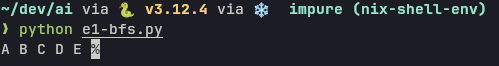
\includegraphics[width=0.5\columnwidth]{./e1-bfs.png}
\end{center}
\item \textbf{Depth-First Search}
  \begin{center}
    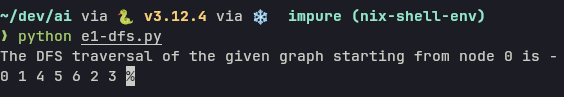
\includegraphics[width=0.5\columnwidth]{./e1-dfs.png}
  \end{center}
\item \textbf{Iterative Deepening}
  \begin{center}
    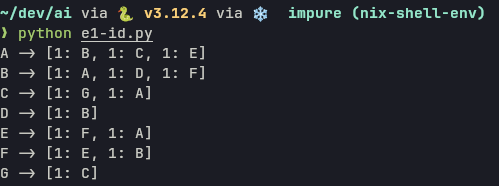
\includegraphics[width=0.5\columnwidth]{./e1-id.png}
  \end{center}
\end{enumerate}
\section{Learning Outcomes}
\begin{enumerate}
  \item Learned about BFS
  \item Learned about DFS
  \item Learned about ID
\end{enumerate}
\end{document}
